\documentclass[12pt]{article}
\usepackage[utf8]{inputenc}
\usepackage{amsmath,amsthm,amssymb,algorithm,hyperref,xcolor}
\usepackage[noend]{algpseudocode}
\usepackage{subcaption}
\usepackage{graphicx}

\title{Distributed Ensembles for Image Classification}
\usepackage{fullpage,comment}
\author{Andrea Burns \and Gavin Brown \and Iden Kalemaj}
\date{\today}
\newcommand{\cP}{\mathcal{P}}
\newcommand{\cD}{\mathcal{D}}
\newcommand{\cR}{\mathcal{R}}
\newcommand{\cS}{\mathcal{S}}
\newcommand{\cN}{\mathcal{N}}
\newcommand{\N}{\mathbb{N}}
\newcommand{\R}{\mathbb{R}}
\newcommand{\E}{\mathbb{E}}
\newcommand{\eps}{\varepsilon}
\newtheorem{theorem}{Theorem}
\newtheorem{conjecture}[theorem]{Conjecture}
\newtheorem{lemma}[theorem]{Lemma}
\newtheorem{claim}[theorem]{Claim}
\newtheorem{corollary}[theorem]{Corollary}
\newtheorem{definition}[theorem]{Definition}
\newtheorem{proposition}[theorem]{Proposition}
\newtheorem{fact}[theorem]{Fact}
\newtheorem{example}[theorem]{Example}
\newtheorem{assumption}[theorem]{Assumption}
\newtheorem{observation}[theorem]{Observation}
\newtheorem{remark}[theorem]{Remark}

\newcommand{\Sec}[1]{\hyperref[sec:#1]{Section\,\ref*{sec:#1}}} %section
\newcommand{\Obs}[1]{\hyperref[obs:#1]{Observation~\ref*{obs:#1}}} %section
\newcommand{\Eqn}[1]{\hyperref[eq:#1]{Eq. (\ref*{eq:#1})}} %equation
\newcommand{\Fig}[1]{\hyperref[fig:#1]{Fig.\,\ref*{fig:#1}}} %figure
\newcommand{\Tab}[1]{\hyperref[tab:#1]{Table\,\ref*{tab:#1}}} %table
\newcommand{\Thm}[1]{\hyperref[thm:#1]{Theorem\,\ref*{thm:#1}}} %theorem
\newcommand{\Fact}[1]{\hyperref[fact:#1]{Fact\,\ref*{fact:#1}}} %fact
\newcommand{\Lem}[1]{\hyperref[lem:#1]{Lemma\,\ref*{lem:#1}}} %lemma
\newcommand{\Prop}[1]{\hyperref[prop:#1]{Prop.~\ref*{prop:#1}}} %property
\newcommand{\Cor}[1]{\hyperref[cor:#1]{Corollary~\ref*{cor:#1}}} %corollary
\newcommand{\Conj}[1]{\hyperref[conj:#1]{Conjecture~\ref*{conj:#1}}} %conjecture
\newcommand{\Def}[1]{\hyperref[def:#1]{Definition~\ref*{def:#1}}} %
\newcommand{\Alg}[1]{\hyperref[alg:#1]{Algorithm~\ref*{alg:#1}}} %algorithm
\newcommand{\Pro}[1]{\hyperref[pro:#1]{Procedure~\ref*{pro:#1}}} %procedure
\newcommand{\Ex}[1]{\hyperref[ex:#1]{Ex.~\ref*{ex:#1}}} %example
\newcommand{\Clm}[1]{\hyperref[clm:#1]{Claim~\ref*{clm:#1}}} %example
\newcommand{\Stp}[1]{\hyperref[step:#1]{Step~\ref*{step:#1}}}
\newcommand{\Ch}[1]{\hyperref[chap:#1]{Chapter~\ref*{chap:#1}}}


\algnewcommand\algorithmicinput{\textbf{INPUT:}}
\algnewcommand\INPUT{\item[\algorithmicinput]}
\algnewcommand\algorithmicoutput{\textbf{OUTPUT:}}
\algnewcommand\OUTPUT{\item[\algorithmicoutput]}

\begin{document}
\maketitle
\section{Links}
\begin{itemize}
	\item Github link: https://github.com/gavinrbrown1/distributed-ensemble-project
	\item Slice name: Project5
\end{itemize}

\section{Introduction}

The general goal of image classification is to determine which of several fixed classes an image belongs to. 
One common benchmark is the CIFAR-10 dataset \cite{cifar10}, which contains 32$\times$32 pixel images of ten different classes: airplanes, automobiles, birds, cats, deer, dogs, frogs, horse, ship, truck.
We've included a selection of these images in Figure~\ref{fig:cifar10_images}.
Image recognition is an important machine learning task, as it is an initial step toward visual scene understanding -- a skill needed to interact with and reason about an environment (use cases include robot assistants, autonomous vehicles, etc).

\begin{figure}
    \centering
    \begin{subfigure}[b]{0.2\textwidth}
        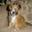
\includegraphics[width=\textwidth]{image0.jpeg}
    \end{subfigure}
    ~
    \begin{subfigure}[b]{0.2\textwidth}
        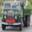
\includegraphics[width=\textwidth]{image3.jpeg}
    \end{subfigure}
    ~
    \begin{subfigure}[b]{0.2\textwidth}
        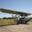
\includegraphics[width=\textwidth]{image5.jpeg}
    \end{subfigure}
    \caption{A few images from CIFAR-10. From left to right: a dog, a truck, and an airplane.}
    \label{fig:cifar10_images}
\end{figure}

Ensembling is a popular way to improve the performance of a machine learning task; an ensemble is a set of different classifiers that are ‘combined’ to make a collective, better decision on the task. 
For a reference see Chapter 14 of Bishop's \emph{Pattern Recognition and Machine Learning}~\cite{bishop}.
%The core idea is that combining many weak learners results in a strong learner. 
%Two common ways to ensemble different classifiers are bagging and boosting. In bagging, classifiers are learned independently, whereas boosting tries to learn new models which succeed in cases that previous classifiers failed. 


In this experiment we distribute 4 independent classifiers across different network nodes (servers) to be used as an ensemble, similar to bagging, in which we take a majority vote of their decisions and use that as the final classification result. This distributed system allows us to investigate latency versus performance benefits when introducing additional classifiers to the ensemble. Lastly, we try hand-crafted caching tools that can act as short-cut decisions, to see the impact on end-to-end delay.

A client wishing to receive classification for an image connects to a manager and sends the image to the manager. The manager then sends copies of the image to the classifiers.




\section{Experimental methodology}

\section{Results}

\subsection{Usage instructions}
\subsection{Analysis results}

\section{Conclusion}

\section{Division of labor}

Andrea, Iden, and Gavin decided on the project topic and wrote the proposal and report together.
All high-level decisions were made together: network topology, communication protocols, experiments, etc.
Much of the coding was done in pairs, as well.
The focus of specific sections were as follows: Andrea created the code to control caching.
Iden wrote the bulk of the socket code that allowed the machines to communicate.
Gavin wrote the code to handle the prediction as well as modeling error and delay on the part of the classifier.


\begin{thebibliography}{1}
    \bibitem{cifar10}
    Krizhevsky, Alex, and Geoffrey Hinton. Learning multiple layers of features from tiny images. Vol. 1. No. 4. Technical report, University of Toronto, 2009.

    \bibitem{bishop}
    Bishop, Christopher M. Pattern recognition and machine learning. Springer, 2006.

\end{thebibliography}



\end{document}
